\section{Methodology}\label{sec:method}

\subsection{Pipeline Overview}

The system is a modular, end-to-end pipeline (Figure~\ref{fig:pipeline_flowchart}) driven by a single YAML configuration: data acquisition, feature engineering, chronological train/test split, model training with PPSO tuning, and multi-metric evaluation. Each stage is an independent Python module.

\begin{figure}[H]
\centering
\begin{tikzpicture}[
    node distance=0.8cm and 1.2cm,
    block/.style={rectangle, draw, fill=blue!8, text width=10em, text centered, minimum height=2.4em, rounded corners=3pt, font=\small},
    data/.style={rectangle, draw, fill=green!8, text width=9em, text centered, minimum height=2.2em, rounded corners=3pt, font=\small},
    arrow/.style={-{Stealth[length=2.5mm]}, thick}
]
\node[block] (config) {1. Load Configuration\\(\texttt{config.yaml})};
\node[data, below=of config] (weather) {Weather Data\\(Open-Meteo API)};
\node[data, right=2.2cm of weather] (demand) {Demand Data\\(EMA CSV)};
\node[block, below=0.8cm of $(weather)!0.5!(demand)$] (merge) {2. Merge \& Validate Data};
\node[block, below=of merge] (preprocess) {3. Feature Engineering\\(16 features)};
\node[block, below=of preprocess] (split) {4. Chronological\\Train/Test Split (80/20)};
\node[block, below left=0.9cm and 1.2cm of split] (train_std) {5a. Train Standard\\Models (LR, RF, XGB, CB)};
\node[block, below right=0.9cm and 1.2cm of split] (train_ppso) {5b. PPSO Optimise\\RF / XGB / CatBoost};
\node[block, below=0.8cm of $(train_std)!0.5!(train_ppso)$] (evaluate) {6. Evaluate All Models\\(6 Metrics)};
\node[data, below=of evaluate] (output) {Results: Leaderboard,\\Plots, Summary};
\draw[arrow] (config) -- (weather);
\draw[arrow] (config) -| (demand);
\draw[arrow] (weather) |- (merge);
\draw[arrow] (demand) |- (merge);
\draw[arrow] (merge) -- (preprocess);
\draw[arrow] (preprocess) -- (split);
\draw[arrow] (split) -| (train_std);
\draw[arrow] (split) -| (train_ppso);
\draw[arrow] (train_std) |- (evaluate);
\draw[arrow] (train_ppso) |- (evaluate);
\draw[arrow] (evaluate) -- (output);
\end{tikzpicture}
\caption{High-level architecture of the electricity demand forecasting pipeline.}
\label{fig:pipeline_flowchart}
\end{figure}

\subsection{Data and Feature Engineering}

Daily national demand (MWh) is obtained from EMA \parencite{ema2025statistics}; four daily weather variables (mean temperature, mean relative humidity, maximum wind speed, cumulative solar radiation) are retrieved from the Open-Meteo Archive API \parencite{openmeteo2025api} for Singapore's coordinates (1.3521$^\circ$N, 103.8198$^\circ$E). An inner join on date yields 1{,}065 observations (February 2023 -- December 2025). Figure~\ref{fig:eda_timeseries} shows the demand and weather series over the three-year period: demand exhibits clear weekly cyclicity and a mild upward trend, while temperature oscillates within the narrow 26--30$^\circ$C tropical band.

\begin{figure}[H]
    \centering
    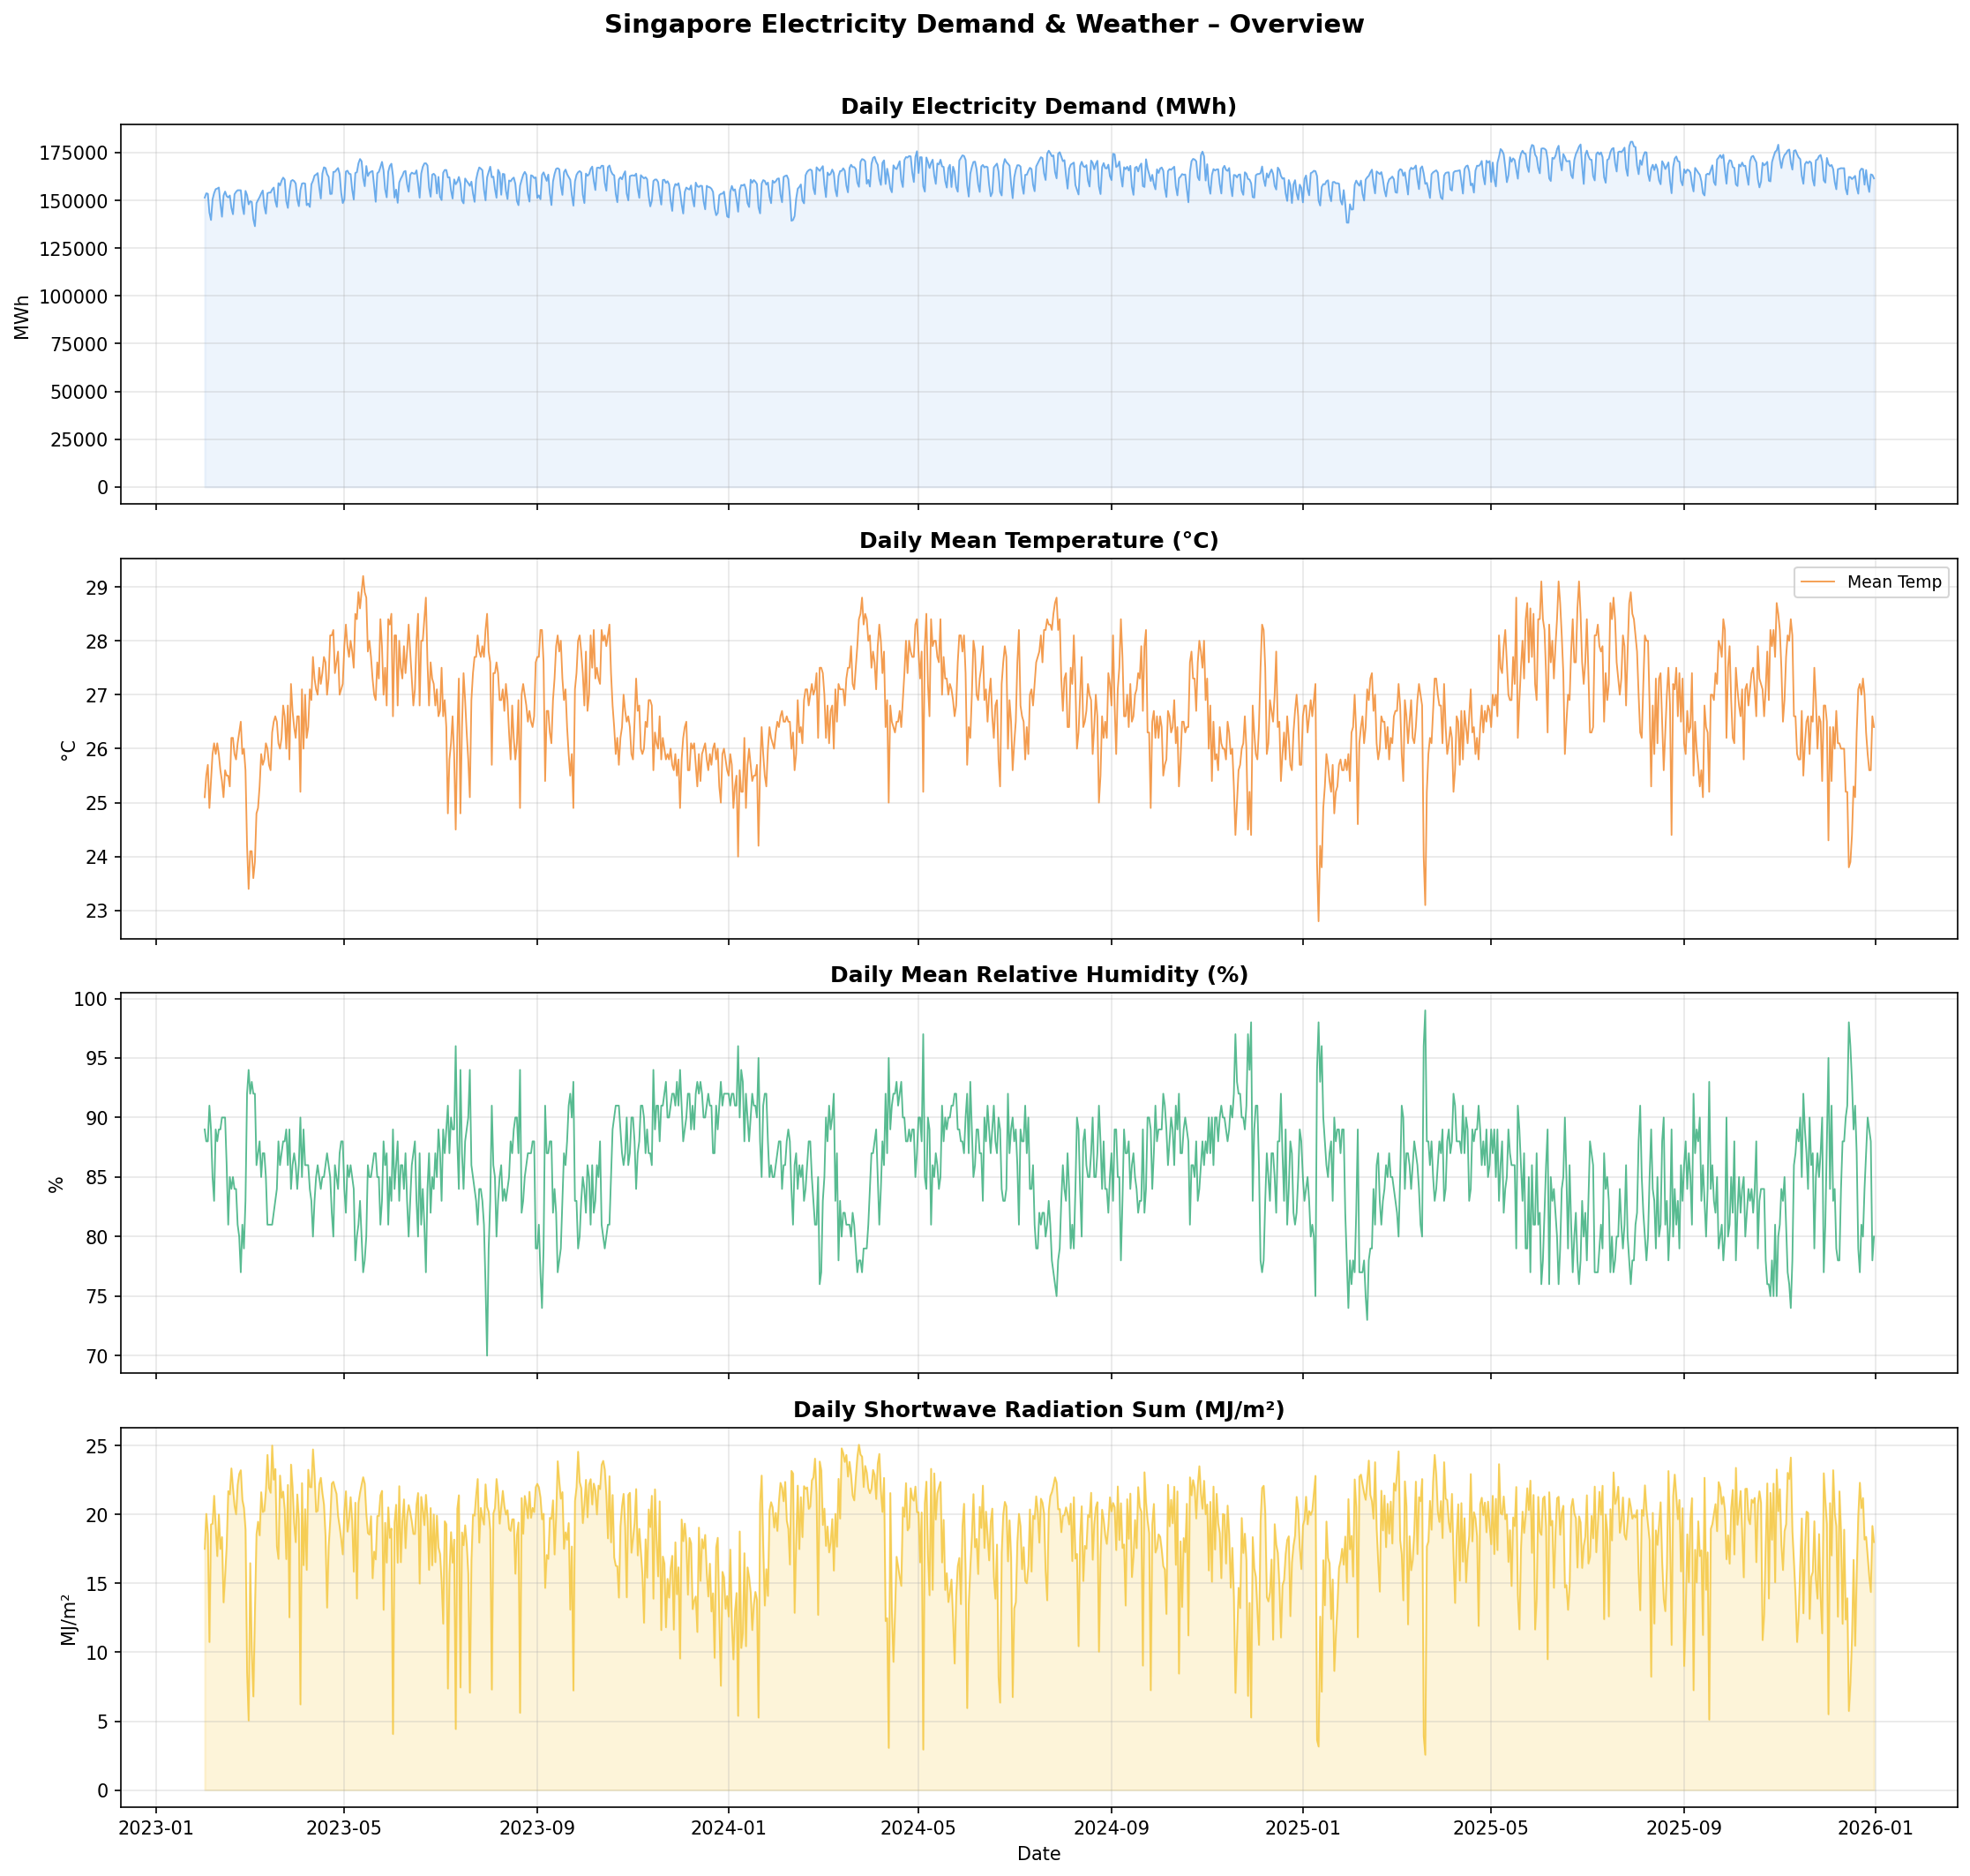
\includegraphics[width=0.92\textwidth]{design/images/eda_time_series.png}
    \caption{Daily electricity demand and weather variables in Singapore, February 2023 -- December 2025.}
    \label{fig:eda_timeseries}
\end{figure}

Sixteen features are constructed across four categories: \emph{weather} (the four raw variables); \emph{derived} --- a Comfort Climate Index, $\mathrm{CCI} = T \times (1 + 0.01 \times H)$, capturing combined thermal stress, plus a season indicator; \emph{temporal} (day-of-week, month, weekend and Singapore public-holiday flags); and \emph{autoregressive} (demand lags at 1 and 7 days; 3- and 7-day rolling means and standard deviations). An 80/20 \emph{chronological} split (852 train / 213 test samples) prevents forward-looking bias; features are standardised only for Linear Regression.

\subsection{Models and Fair Tuning Protocol}

Eight configurations are compared: a Lag-1 baseline, Linear Regression, and default Random Forest, XGBoost, and CatBoost, plus PPSO-tuned variants \textbf{RF-PPSO}, \textbf{XGB-PPSO}, and \textbf{CatBoost-PPSO}. The central methodological decision is to apply PPSO to \emph{every} tunable model under an \emph{identical} budget, rather than only to CatBoost as in the reference study \parencite{zhang2023catboostppso}. This isolates each algorithm's intrinsic merit from the benefit of tuning.

PPSO was selected for three pragmatic reasons: (i) it is \emph{parameter-free}---the phasor angle adaptively balances exploration and exploitation, avoiding meta-tuning of the optimiser itself, which would re-introduce experimenter bias; (ii) its periodic velocity modulation suits the non-convex, expensive hyperparameter landscape where each fitness call requires several full model trainings; and (iii) it was validated against six meta-heuristics in the closest prior study \parencite{zhang2023catboostppso}. Mathematical details follow Ghasemi et al.\ \parencite{ghasemi2019ppso} and are not repeated here.

Each model's four-dimensional search space covers its most sensitive hyperparameters (Table~\ref{tab:search_spaces}). The shared budget is 15 particles $\times$ 20 iterations with early stopping after 5 stagnant iterations; fitness is the mean RMSE over 3-fold \texttt{TimeSeriesSplit} cross-validation on the training set only (Figure~\ref{fig:ppso_workflow}). All seeds are fixed to 42.

\begin{table}[H]
\centering
\caption{PPSO hyperparameter search spaces (identical budget for all models).}
\label{tab:search_spaces}
\small
\begin{tabular}{@{}lllll@{}}
\toprule
\textbf{Model} & \multicolumn{4}{c}{\textbf{Tuned hyperparameters (bounds)}} \\
\midrule
Random Forest & trees (100--800) & depth (4--25) & min split (2--20) & min leaf (1--10) \\
XGBoost & trees (100--1000) & depth (3--10) & learn.\ rate (0.01--0.2) & $L_2$ (1--20) \\
CatBoost & iterations (100--800) & depth (4--10) & learn.\ rate (0.01--0.2) & $L_2$ (1--20) \\
\bottomrule
\end{tabular}
\end{table}

\begin{figure}[H]
\centering
\begin{tikzpicture}[
    node distance=0.55cm,
    block/.style={rectangle, draw, fill=blue!8, text width=13em, text centered, minimum height=2.2em, rounded corners=3pt, font=\small},
    decision/.style={diamond, draw, fill=orange!12, text width=6.5em, text centered, aspect=2, inner sep=1pt, font=\small},
    arrow/.style={-{Stealth[length=2.5mm]}, thick}
]
\node[block] (init) {Initialise $N$ particles with random positions \& phases};
\node[block, below=of init] (eval) {For each particle: train candidate model with 3-fold TS cross-validation};
\node[block, below=of eval] (fitness) {Fitness = mean validation RMSE};
\node[block, below=of fitness] (update_pb) {Update personal / global best};
\node[block, below=of update_pb] (ppso_update) {PPSO velocity, position, and phase angle update};
\node[decision, below=of ppso_update] (converge) {Converged or max iter?};
\node[block, below left=0.9cm and -1cm of converge] (final) {Train final model with best hyperparameters on full training set};
\draw[arrow] (init) -- (eval);
\draw[arrow] (eval) -- (fitness);
\draw[arrow] (fitness) -- (update_pb);
\draw[arrow] (update_pb) -- (ppso_update);
\draw[arrow] (ppso_update) -- (converge);
\draw[arrow] (converge) -- node[right, font=\small]{Yes} (final);
\draw[arrow] (converge.east) -- ++(1.4,0) |- node[near start, right, font=\small]{No} (eval.east);
\end{tikzpicture}
\caption{PPSO hyperparameter optimisation workflow (applied identically to RF, XGBoost, and CatBoost).}
\label{fig:ppso_workflow}
\end{figure}

\subsection{Evaluation Metrics}\label{sec:eval_metrics}

Following Zhang et al.\ \parencite{zhang2023catboostppso}, six metrics are computed on the held-out test set: MAE, RMSE, MAPE, and RAE (errors; lower is better) plus $R^2$ and the Willmott Index (WI) \parencite{willmott1982validation} (agreement; higher is better). WI is included for its robustness to outliers relative to $R^2$.

\subsection{Web Portal}

The best model is deployed via a lightweight portal: a FastAPI backend loads the serialised model and exposes REST endpoints (\texttt{/api/summary}, \texttt{/api/range}, \texttt{/api/predict}, \texttt{/api/forecast}), and a React/Vite frontend offers a \emph{History Report} page (retrospective accuracy over a chosen period, Figure~\ref{fig:dashboard}) and a \emph{Demand Trends} page (forward outlooks driven by live Open-Meteo weather forecasts).

\begin{figure}[H]
    \centering
    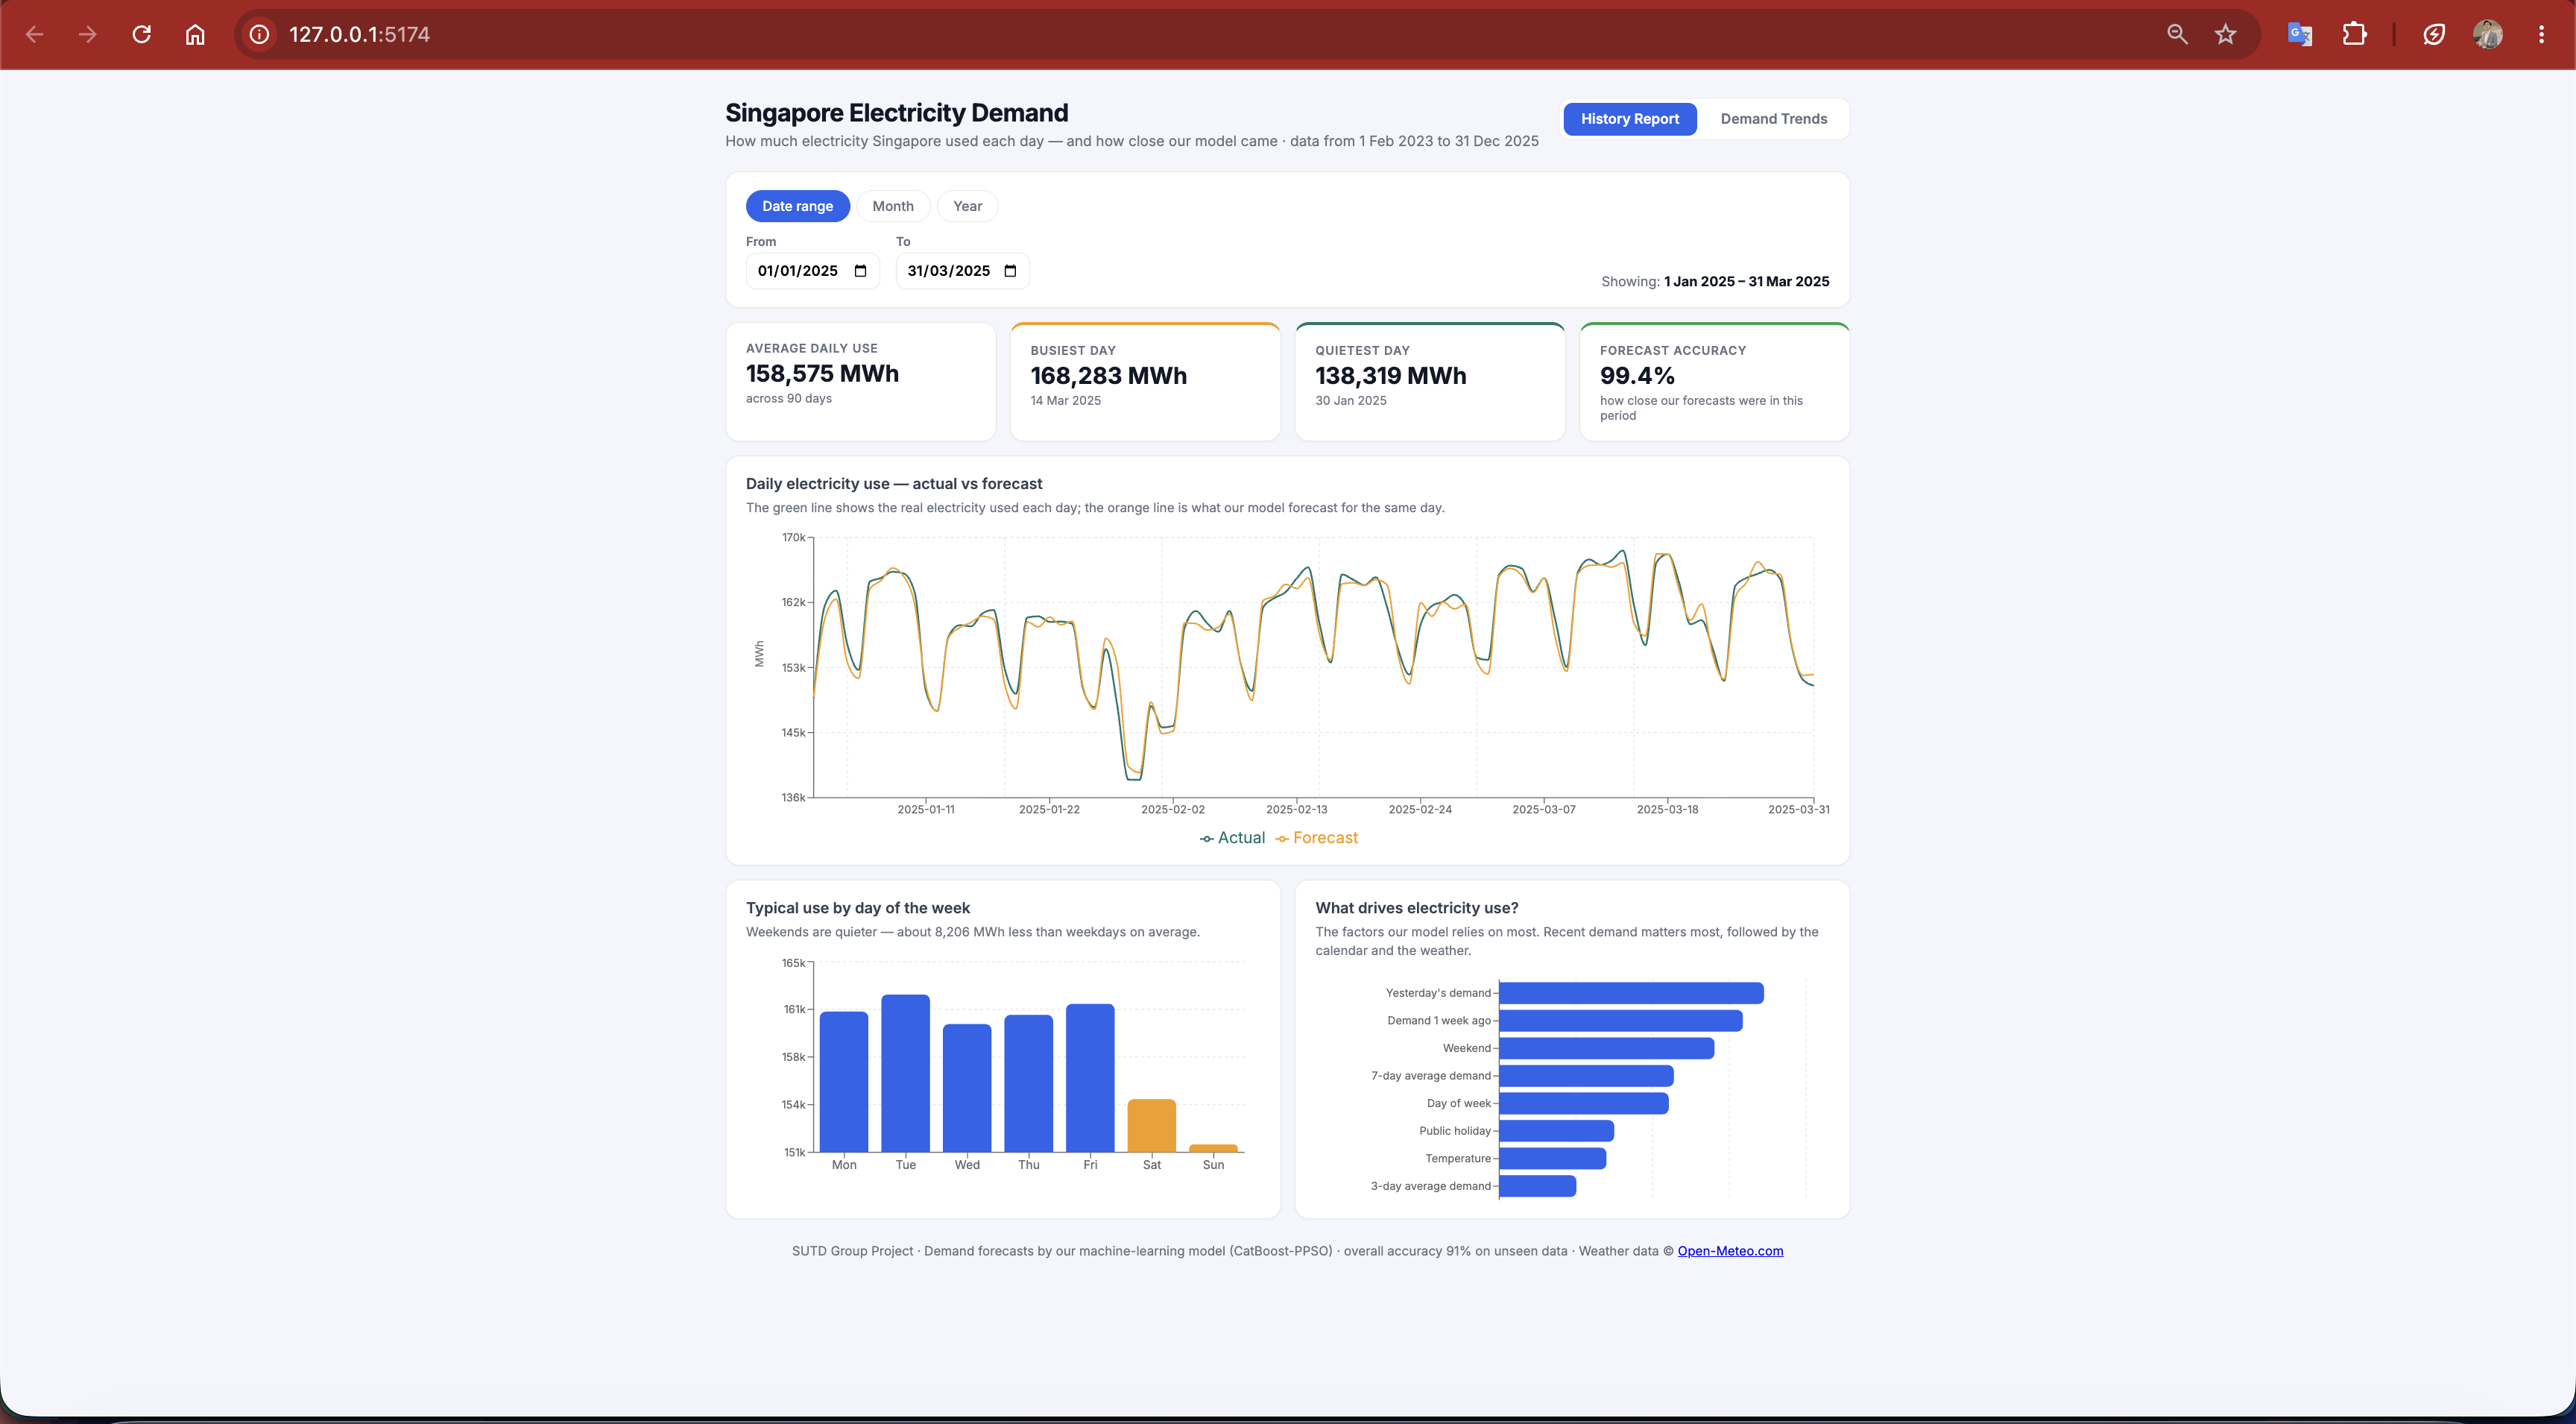
\includegraphics[width=0.88\textwidth]{impl/images/dashboard_history.png}
    \caption{History Report page of the web portal: actual vs.\ predicted demand and summary statistics for a user-selected period.}
    \label{fig:dashboard}
\end{figure}
